% !TeX spellcheck = en_GB
\chapter{Results}

\section{Demonstration of conventional polarisation microscopy}
\label{sec:conventional pol}

\begin{figure}
	\centering
	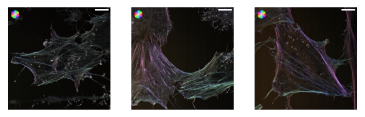
\includegraphics{conventional_pol.pdf}
	\caption{
		Polarisation microscopy images of three different cells. The colour wheel indicates the direction of polarised light corresponding to a certain colour. Scale bars \SI{10}{\mu m}. \todo{Get a camera view of with GFP and DAPI signals, see 21-02-05}
	}
	\label{fig:conventional pol}
\end{figure}

Even though we can't use polarisation on the detection side yet, we can already make polarisation images by varying the angle of excitation polarisation. As a proof of concept, I imaged the sample described in \autoref{sec:samples}, stepping the excitation light from \ang{0} to \ang{170} in steps of \ang{10}. Applying the algorithm detailed in \autoref{sec:pol analysis} to three different ROIs resulted in \autoref{fig:conventional pol}. As expected, vertically oriented fibres are excited by horizontal polarisation \cite{Spira2017}.

I also included power law scaling of the saturation (degree of polarisation) and value (total brightness) in the visualisation algorithm. These serve to adjust the brightness and contrast of the figure, as shown in \autoref{fig:power law exponents}.

\begin{figure}
	\centering
	\includegraphics{conventional_pol_exps.pdf}
	\caption{
		The effect of the exponents $ \alpha_s $ (tuning saturation) and $ \alpha_v $ (scaling brightness) on an image.
	}
	\label{fig:power law exponents}
\end{figure}

\todolist{
	\item I could plot some histograms and stuff, of the polarisation distribution, but I guess that only really makes sense if I can actually make a substantial comment about it.
	\item sSTED + polarisation
} 

\section{Polarisation-resolved STED microscopy}

In this section, I will detail how we implemented the pSTED scheme detailed in \autoref{sec:methods psted} and how we verified that it is working as predicted \todo{rephrase if conclusion is that it doesn't work ye}. The first step is to manipulate the polarisation of the depletion beam. Then I can do experiments on unpolarised and polarised controls (beads and Yersinia samples).

To get control of the light polarisation, the first step was to mount two new waveplates in the beam path. They were mounted after the SLM. A HWP was mounted inside a rotational stage and a QWP went in a cage system attached to the rotational stage, such that it is always aligned with the HWP, but that its rotational angle is fixed. The first step was to find the angle of the QWP that maximised the linearity of the light polarisation at the sample. This was simply done by placing a polariser and a power meter at the sample and rotating them to characterise the polarisation of the depletion beam. I did this a couple of times, from which we concluded that the optimal angle for the QWP was 15°. Next, I had to find the angle of the HWP at which the depletion beam is vertically polarised. In that position, the depletion beam has a polarisation parallel to the excitation lasers (at 0°). This turned out to be 38.4°. See \autoref{fig:psted hwp offset}. At a linearity of $ I_{max}/I_{min} = 5.47 $ (corresponding to an ellipticity $ \chi = \ang{10.3} $ )\todo{depends on definition of $ \chi $ again}, the polarisation of the linearised pSTED beam is comparable in quality to the 640 laser.

Now that we have control over the beam polarisation, we can check how the added waveplates influence the PSF. In \autoref{fig:psted psfs}, the PSF is shown for different polarisation directions. There are a number of conclusions we can draw from this data.  Firstly, the PSF is not radially symmetric any longer, even though the SLM was set to Gaussian mode. In particular, the ellipse orientation is parallel to the light polarisation, so we see the PSF rotating as we change the polarisation. This can be explained by the fact that a lens interacts differently with light polarised along different directions \cite{Egner2020}. This is the reason one should only use linearly polarised excitation light when performing polarisation microscopy.

Other effects of the polarisation include the following: the intensity of the depletion beam varies as a function of the polarisation angle. This is probably due to linear dichroism present in the optical elements between the waveplates and the sample. That is to be expected, but should be accounted during either image acquisition or analysis. Furthermore, the eccentricity of the ellipse has a slight dependency on the polarisation angle, and the maximum of the PSF moves a little: up to \todo{?} nm from its mean position. Fortunately this is a quite a bit below the diffraction limit for 775 nm light, i.e.~around 400 nm. \todo{Plot this data!}

\todo{NOTE THAT WE HAVE TO ROTATE THE HWP BACKWARDS!!!!!!!!}

Finally, we can perform pSTED on some control samples. I used two different ones: a sample of non-polarised beads and the cell sample shown earlier. Isotropic beads are useful, since we can determine the polarisation of emitted light by selectively activating fluorophores of a particular orientation with the polarisation of the excitation light. This process is called photoselection. When these beads are excited with circularly polarised light, fluorophores of all orientations should be activated equally, and the polarisation of the depletion beam should not matter. In the case of linearly polarised excitation light, on the other hand, depletion should be more efficient when its polarisation is aligned with the excitation beam. This can be verified by increasing the depletion power: when the beams are aligned, then the remaining fluorescence signal should drop faster than when they are not, as predicted by \autoref{eq:psted integral}. \autoref{fig:psted beads} shows that this is indeed the case. While there is some variation in the depletion rate under circular excitation, it can not be explained by the theory and seems random, unlike the case of linear excitation. There, depletion goes fastest when the beams are aligned, slower when there is a 45° angle between them, and slowest when they are orthogonal. If the depletion beam was more linearly polarised (i.e. had a lower $ \chi $), then this effect would be even more pronounced.

\begin{figure}
	\centering
	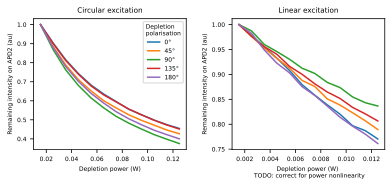
\includegraphics{psted_beads.pdf}
	\caption{
		Dependency of surviving fluorescence on intensity and polarisation of depletion beam. \textbf{Left:} circular excitation. \textbf{Right:} linear excitation at 0° (vertical). \todo{Planning to do a number of repeats to get rid of noise in this figure.}
	}
	\label{fig:psted beads}
\end{figure}

\todo{pSTED results in cells. Mention spacer channels. Mention that pSTED intensity shouldn't be too high, otherwise you'll never see anything.}




























